% !TeX spellcheck = <none>
% !TeX program = pdflatex
% !TeX TXS-program:bibliography = txs:///bibtex
% !BIB program = bibtex

%% LMU-MI-HS-Template
%% This template is an adaptation of the IEEE InfoVis/Vis format
%% http://www.cs.sfu.ca/~vis/Tasks/camera_tvcg.html
%% Last update: Bastian Pfleging, 05.2016

\documentclass[journal]{vgtc}                % final (journal style)
\usepackage[english]{babel}
\usepackage{mathptmx}
\usepackage{graphicx}
\usepackage{times}
\usepackage[hyphens]{url}
\usepackage{float}
\usepackage[hidelinks]{hyperref}
\usepackage[nolist]{acronym}

\usepackage[backend=bibtex, style=numeric, isbn=true, doi=true, maxnames=99]{biblatex}
\addbibresource{literature.bib}

\DeclareGraphicsExtensions{.pdf,.jpg,.pdf,.mps,.png}
\graphicspath{{img/}} 

\usepackage[official]{eurosym}

\normalfont

\begin{acronym}[Bash]
	\acro{QR}{Quantified Relationship}
	\acro{QS}{Quantified Self}
	\acro{GDPR}{General Data Protection Regulation}
	\acro{EU}{European Union}
	\acro{NCR}{Natural Conception Regulation}
	\acro{IPV}{Intimate Partner Violence}
\end{acronym}

%% Paper title.
\title{Intimate Data in Relationships: Tracking, Sharing, Surveillance - Personal Boundaries?}

%% Put your name here
\author{Diana Irmscher}
\authorfooter{
\item
  Diana Irmscher is studying Media Informatics at the University of Munich, Germany, E-mail: d.irmscher@campus.lmu.de
\item
  This research paper was written for the Media Informatics Advanced Seminar 'Advanced Seminar in Media Informatics',
  2018
}


%% Abstract section.
\abstract{
	% One or two sentences providing a basic introduction to the field, comprehensible to a scientist in any discipline.
	Self-Tracking and representing the self in online communities and websites has become commonplace.
	% Two to three sentences of more detailed background, comprehensible to scientists in related disciplines.
	The Quantified Self Movement has gained more and more popularity. There are groups aroud the world, e.g. \textit{The Munich Quantified Self Meetup Group}.
	Nowadays many people use devices and smartphone applications to simplify the everyday life and gain new insights, not only for sports activities, but also in interpersonal relationships.
	% One sentence clearly stating the general pr                                    oblem being addressed by this particular study.
	This paper considers why people gather, search, track and share intimate data in romantic relationships. Further it is investigated how they perceive these data and how this affects the perception in context to social life.
	% Two or three sentences explaining what the main result reveals in direct comparison to what was thought to be the case previously, or how the main result adds to previous knowledge.
	It can be shown that the perception of what intimate data are is very subjective and depends on different circumstances. People gather, search, track and share their intimate data in nearly all states of an interpersonal, romantic relationship. They are not always aware of what exactly is capture by technologies, nor are they aware of the consequences that can result. The role of third parties can be problematic, because they have commercial interests in these data.
	
	% One or two sentences to put the results into a more general context.
	Everyone should reconsider the use of such technologies. It is necessary to investigate in further work what influence the use of such technologies has on relationship life.
	
	% Two or three sentences to provide a broader perspective, readily comprehensible to a scientist in any discipline, may be included in the first paragraph if the editor considers that the accessibility of the paper is significantly enhanced by their inclusion. Under these circumstances, the length of the paragraph can be up to 300 words. (This example is 190 words without the final section, and 250 words with it).
}

%% Keywords that describe your work.
\keywords{intimate data, quantified relationship, surveillance, self-tracking, self-quantification, data ethics, privacy, love}

%%%%%%%%%%%%%%%%%%%%%%%%%%%%%%%%%%%%%%%%%%%%%%%%%%%%%%%%%%%%%%%%
%%%%%%%%%%%%%%%%%%%%%% START OF THE PAPER %%%%%%%%%%%%%%%%%%%%%%
%%%%%%%%%%%%%%%%%%%%%%%%%%%%%%%%%%%%%%%%%%%%%%%%%%%%%%%%%%%%%%%%%

\begin{document}

\firstsection{Introduction}

\maketitle

% ------------------------------------------------------------------------------
%
% This is only an exemplary structure for your paper! Feel free to change the names of the sections
% and subsections! 
%
% ------------------------------------------------------------------------------
\label{sec:introduction}
% Move 1: Establishing a Territory

% Step 1: Claiming importance and/or
% Step 2: Making topic generalization(s) and/or
% Step 3: Reviewing items of previous research
In the century of digitalization there are many opportunities offered to perceive the self in everyday life in a different way as before. Tracking and quantifying the self, the body an also other aspects in life is commonly used as showed in \cite{kelly2017inevitable}. Nowadays many people are engaged in tracking such data like heartbeat, sleeping pattern and other quantifiable data. They are tracking and also sharing this information with others, like friends or like-minded people. 

% Move 2: Establishing a Niche

% Step 1A: Counter-claiming or
% Step 1B: Indicating a gap or
% Step 1C: Question-raising or
% Step 1D: Continuing a tradition

But there are many different types of data which can be tracked. Superficially, such data like heartbeat or sleeping pattern does not seem apprehensive when tracking and sharing these with others, but how about data in intimate relationships and sexual behaviors?

% Move 3: Occupying the Niche

% Step 1A: Outlining purposes or
% Step 1B: Announcing present research
In this work it is investigated how people use techniques for collecting, tracking, storing and sharing of intimate data in romantic relationships. Techniques in this field also called \acl{QR} techniques. In addition to tracking and sharing, surveillance also plays a key role, which is considered.
Therefore, the following questions will be answered by reviewing literature and studies in this scientific field:
%TODO: Answering these questions in conclusion
 \begin{description}
 	\item[RQ1:] What data is perceived as intimate? In what circumstances?
 	\item[RQ2:] Why do people track intimate data in relationships?
 	\item[RQ3:] What do they do with, e.g. tracking, storing, sharing and discussing and with whom?
 	\begin{enumerate}
 		\item Do they over-trust the tracked data?
 		\item How do they perceive their tracked data?
 	\end{enumerate}
 \end{description}
For answering the questions mentioned above a research of literature and studies on collecting, tracking and sharing intimate data in romantic relationships is carried out. In Addition, some articles and reports by users of tracking and other technologies are also used for finding answers, e.g. the report by Duportail \cite{Duportail2017} about the data which tinder collect over a period of time.

% Step 2: Announcing principal findings
Intimate data are searched, collected, tracked, stored and shared in every part of relationship, from the beginning until to termination.
The different types of intimate data were collected from \textit{Facebook} and \textit{Tinder} and tracked by \acl{QR} technologies, for example to quantify sexual activities or measuring menstrual cycle.
The several types of intimate data are obtained from different sources. At the beginning of a relationship, data are gathered from Facebook, Tinder and other soical networks.
At the point the relationship is "established", other technologies become more relevant, e.g. \acl{QR} technologies, to quantify sexual activities or measuring menstrual cycle of the partner, to gain more details about the mood.
If a romantic relationship is broken off, social networks and \acl{QR} technologies can be abused, e.g. to stalking the ex-partner, or even harm. 
The usage of all these digital helpers in intimate relationships is always associated with a certain risk.
Often, default security precautions are insufficient for specific situations, e.g. as in the dissolution of a relationship. 
Frequently users are not aware about the type and scope of intimate data which collected and tracked by their own devices (e.g. the smart phone), and which my be accessible by others like the ex-partner or third parties.

% Step 3: Indicating research article structure
In section \ref{sec:terms_of_definition} the term \textit{intimate} is defined by gathering different definitions related \acl{QR}-technologies and intimate surveillance.
In section \ref{sec:life_course} the so called life course of intimate data is defined including four conditions in which an intimate relationship could be.
The following section \ref{sec:consideration_life_course_conditions} describes the conditions with regarding to the intimate data that are searched for, tracked, stored and shared in these circumstances.
In section \ref{sec:risks} the risks related to the use of such technologies in a romantic relationship is investigated.
Section \ref{sec:conculsion} includes a summarization of the work with a short view for future steps.

\section{Terms of Definition}
\label{sec:terms_of_definition}
In this section the term \textit{intimate} is defined. Due to this it is considered which data is perceived as intimate and in which circumstances.
Answering the first research question in this work is not as easy as it seems. Therefore, several definitions from different source are collected.

The perceiving of what is intimate depends on several factors.
In general it has to be differentiate between the culture, how a human is perceiving the self and which factors are shaping the sociocultural live \cite{carrithers1985category}. It is not possible to consider all well-known cultures in this work, therefore the focus is limited to the scrutiny of the western civilization. 
\begin{figure}[htb]
	\centering
	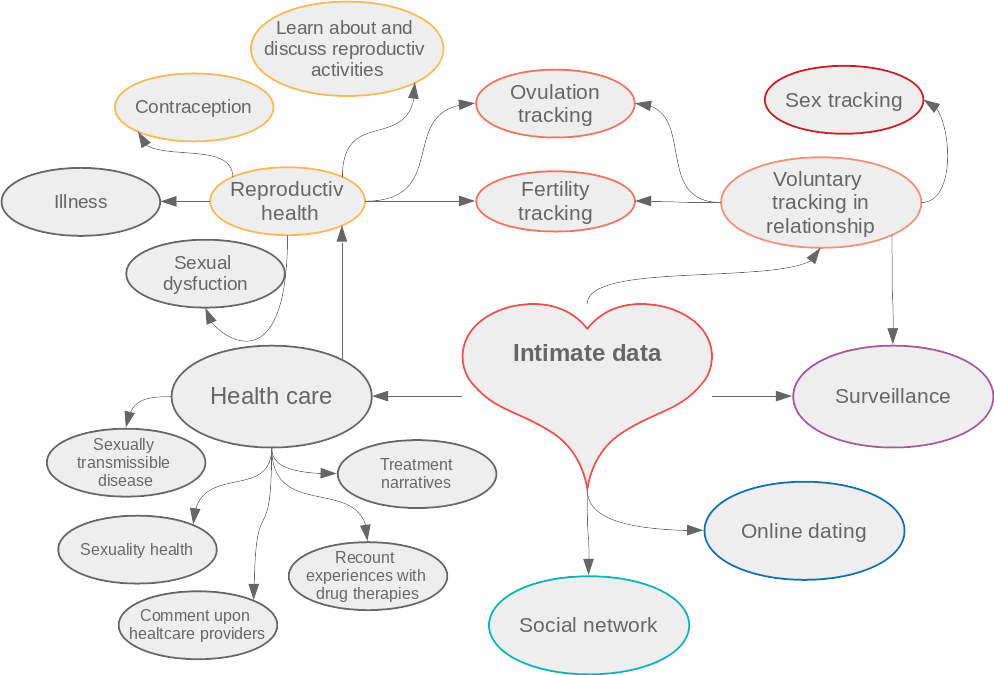
\includegraphics[width=\linewidth]{img/cluster_heart.png}
	\caption{Visualization of possible intimate data, which are arising from using such digital technologies.}
	\label{fig:cluster}
\end{figure}
In the western civilization or rather in the \ac{EU} privacy and data security takes up more attention, even since the \ac{GDPR} is applied \cite{albrecht2016gdpr}.

However, the state of a person in the society is defining the personal perception of privacy and data security, and the personal view as well. What is perceived as intimate depends on this factors.
But these can not be defined in a few sentences, the topic is to complex and not measurable. Furthermore, it is subjective. For the individual, the perception of whether data are intimate or not is different. 
Several works are focused on intimate data in different contexts. Although, a clear definition of which data is intimate or what people perceive as intimate is not clearly defined. Due to this, some descriptions are summarized to give a rough outline.

The focus in Danaher et al. \cite{doi:10.1080/15265161.2017.1409823} is on intimate interpersonal relationships. In this work no clear definition is presented. They argument that it does not need a precise definition to get an understanding of intimate relationships. However, to describing a romantic relationship the authors in this work are writing the following:

\begin{quote}
	[...] we trust that most readers' intuitive sense of those terms [..] will be adequate for our arguments to make sense". 
	That said, romantic relationship might usefully be thought of as a cluster concept, with paradigmatic examples in the middle, and less paradigmatic examples clustered around it, each one different along various dimensions (e.g., the degree to which sexual interaction is central to the relationship).
\end{quote}

If it possible to define an intimate or romantic relationship about such a way, this concept will also fit for the term intimate. We can build a cluster categories of intimate data, which are assigned to corresponding activities, e.g. fertility tracking.

In figure \ref{fig:cluster} several topics related to the term intimate data are collected and brought in relation to each other. At this point it must be emphasized that this does not cover the complete field, in which intimate data would be collected, tracked, shared and so on. Rather it is an summarization of terms and descriptions from Levy \cite{levy2014intimate}, Danaher et al. \cite{doi:10.1080/15265161.2017.1409823}, Lupton \cite{doi:10.1080/13691058.2014.920528} and more. 

The idea to use an cluster concept can be thought of one step further. The sensitivity or level of intimate data could be arranged in some sort of data hierarchy. Form IT-Security Management it is known to evaluate risks by assigning a probability and to classify accordingly (see documentation of Federal Office for Information Security (BSI) \cite{bsi}). In this table I want to classify the data summarized above based on their sensibility.
%TODO: Tabelle über die oben genannten Daten einfügen mit Einstufung; Stufung bestimmen

To give another understanding of what is meant with \textit{intimate} in this paper I want to quote a paragraph form Lupton \cite{doi:10.1080/13691058.2014.920528}, which describes an Application for mobile phones:
\begin{quote}
	The	Glow app brings male partners into the equation by sending them a digital
	message when their partner is in her fertile period and reminding them to bring her flowers	[...]. This app also tracks menstrual and ovulation indicators, as well as asking women to enter details of their sexual encounters, including sexual positions used, whether or not they had an orgasm and whether they experienced emotional or physical discomfort during sex. It employs the aggregated data from other users to refine predictions of ovulation and fertility for the individual user. [...]
\end{quote}
This paragraph describes a sort of tracking which also called \textit{intimate tracking} (defined by \cite{doi:10.1080/15265161.2017.1409823}).

We can also find intimate data also in other contexts, e.g. as mentioned above in health care.
%TODO: finde Quellen zu Aufsätzen intimer Daten in Verbindung mit Drogensucht
But the focus in this paper is on intimate data in relationships, therefore it is referred to the figure \ref{fig:cluster} above. This should give a general understanding of the context. 


\section{Life course of intimate relationships}

Levy \cite{levy2014intimate} has defined a so called \textit{life course of intimate relationships}. This course includes four conditions of romantic relationships (see Figure \ref{fig:live_course}). Each condition is colored from colors from figure \ref{fig:cluster}. Here, the connection to the individual topics should be roughly indicated. The transitions in content are sometimes fluid.
\begin{figure}[htb]
    \centering
	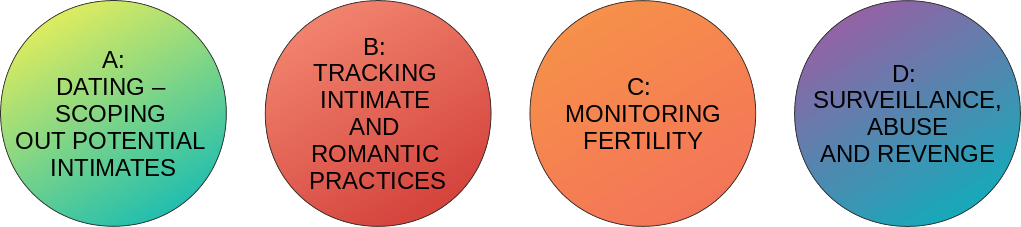
\includegraphics[width=\linewidth]{img/life_course_of_intimate_surveillance.png}
	\caption{The life course of intimate surveillance. Each condition is co}
	\label{fig:live_course}
\end{figure}

In each of these conditions (potential) partners can use technologies for different purposes.

Condition \textbf{A} stands for the beginning of a potential relationship. The partners know each other or would like to know each other. At this point, there is an interest from one or both sides. The aim is to learn more about the other person, to check their identity and social life.

In condition \textbf{B} the partners are already in a relationship or something appropriate. At this point, it should be emphasized that this condition includes all sorts of relationships that are understood as such. For a concretely definition what a (romantic) relationship means see Danaher et al. \cite{doi:10.1080/15265161.2017.1409823} or \ref{sec:terms_of_definition}. In this condition the partners know each other better and have an increased (mutual) interest. There were other forms of contact, possibly sexual contact.

In condition \textbf{C} there is usually an established relationship (but that does not have to be the case, there maybe exceptions). The couple exercises sexual activities, deals with contraceptive measures (together) or plans to start a family.

Condition \textbf{D} contains the surveillance of the partner, also abuse (of data) and revenge. Describing this condition is complicate. 
It can be a relationship that has already ended. The partners therefore have a relationship to each other based on their previous history. This can be different (as in the other states). More generally, this condition maybe arise from problems in the relationship, due to interpersonal conflicts oder something else. But it may also be a state or point in the relationship which is fine for both partner (that refers to the surveillance). This will be discussed later on.

Since relationships are complex and individual, the single conditions are not interconnected \cite{sassler2010partnering}. Also this is not the focus of this work. The descriptions above only should give an idea of what the conditions mean for the following section \ref{sec:consideration_life_course_conditions}, in which all conditions will be discussed in detail.


\section{Consideration of each condition in life course of intimate relationships}
\label{sec:consideration_life_course_conditions}
This sections is about how technologies like social networks, search engines, tracking devices and applications for the smart phone may be applied in a relationship.
For that each condition is investigated for the type of data that can be searched, collected, tracked and shared by the user or others.
The conditions are treated in separate paragraphs, which summarize the intimate data that may be collected, tracked and monitored. Also it is about how these data are perceived by the user and how the data affect the user's perception.

\subsection{Condition A: Dating - Scoping out potential intimates}
\label{subsec:A}
At the beginning of a potential relationship one wants to know more about the other person of one's own interest. Due to this, one collects data about this person. 
\subsubsection{Searching for information}
A way to get relevant information about another person one is interested in, is to use a standard social network like Facebook \footnote{\url{www.facebook.com}} or a search engine like Google Search \footnote{\url{www.google.com}}.
Monitoring a person on Facebook is known as \textit{Facebook stalking} \cite{levy2014intimate}. To stalk on Facebook without getting caught, many articles have been written about \cite{sueddeutsche_fb_stalking}. With the Website stalkscan.com \footnote{\url{https://stalkscan.com}} it is possible to get all public entries from a person's Facebook profile site by only one mouse click. While it can only show what is already public, it makes it easier to stalk another person quickly.
This website as a tool to spy on information about another person avoids making an involuntary like when clicking through the photos on Facebook.
With the Google Search one can find information about another person which are available on the web, as mentioned above. This is commonly known as \textit{google someone}. With this method is it possible to get information from every source which is findable for the search engine \cite{nolan2005hacking}. There are also many articles how to \textit{google someone}. In Google suggestion are made based on common search items, as shown in figure \ref{fig:how_to_google_someone}.

\begin{figure}[htb]
  \centering
  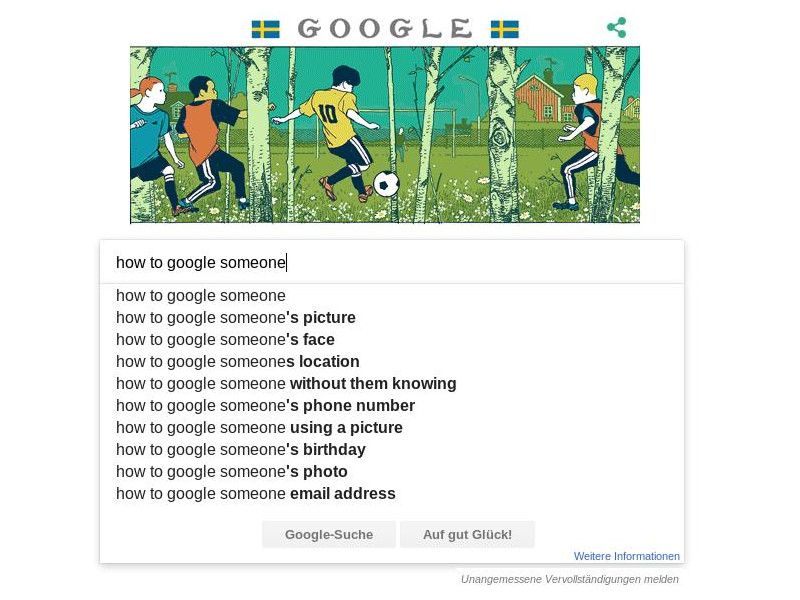
\includegraphics[width=\linewidth]{img/how_to_google_someone.jpeg}
  \caption{Google Search suggestions for \textit{google someone}, (screenshot taken on 07.07.2018 on \url{www.google.com})}.
  \label{fig:how_to_google_someone}
\end{figure}

\subsubsection{Creating and providing information}
The topic in condition A is not only searching for data about another person, but also create such data. Levy \cite{levy2014intimate} wrote about the application Lulu as tool to create data for use in prospective relationships. The focus of this application is on campus life. Lulu gives young women the opportunity to review male students and friends, with which they are connected on Facebook. The review contains information in relation to humor, manners, look and style, sex and kissing. The review given by the female users is anonymous. In the first version of Lulu, users could review each male friend which they had on Facebook. But after the reviewed male Facebook users complained and expressed privacy concerns, a review can only be committed for male users who have explicitly allowed this.

Further, services that combine online dating with user's geographical location are well known. Tinder is a widespread location-based dating service. The smartphone application shows potential "dates" or partners with common interests (e.g. romantic relationship) near to the user's location or next holiday destination \footnote{\url{https://tinder.com}}. By showing the user several profiles he/she can decide to swip right for a \textit{like}. If the other person does also a right swip, it is a \textit{match}. Now the user can exchange messages, e.g. to arrange a date. The principle sounds easy. But by using the Tinder application, a huge amount of intimate data are collected. 
Tinder is connected to Facebook and Instagram, a photo-sharing social networking service, owned by Facebook. Considering this fact there is a huge commercial interest to assume.

Duportail, a French journalist, demanded access to her personal data after four years of using the Tinder application \cite{taylor2009privacy}. In the \acs{EU}, she has the legal means to request this data, using the European data protection law. The response was a more that 800 pages report including different types of data like Facebook likes, information about education, age-rank of men she was interested in, number of Facebook friends, when and were every online conversation with her matches happened, also interests and jobs, pictures, sexual preferences. The list contains a huge amount of intimate data. In her article Duportail wrote that she was surprised by how much information she was voluntarily disclosing.
In \cite{taylor2009privacy} this is called \textit{secondary implicit disclosed information}. Firms have an increasing interest in gathering personal data from user's activities. This results in a trade-off for the user - use the system and accept privacy concerns due to the commercial interest from the provider, or abstain the service.

Despite all concerns, users reveal their data quickly, as shown in Tait et al. \cite{tait2015hello}. 
The study showed that users who tend to gain confidence quickly, therefore, also more quickly reveal more information. In addition, it showed that higher profile activity increases the amount of information desired. 
That means, users who maintain an active profile and present activity also receive more and higher information from other user's rather than users of profiles that provide barely information. The disclosure of information is determined in part by the personality of the user and the context in general. This affects how users surround their data online and with strangers. They found out that in only 6 - 10 minutes a user can extract the full name and date of birth from a conversation. With these information it is easy to get further data about the person via Google Search and Facebook.

Nandwani et al. \cite{10.1007/978-3-319-61542-4_32} examined how quickly users reported their data to strangers and, above all, which data. For the study, an automatism was developed to contact 100 Tinder users. The study was a single blind study, so users did not know at the moment that they were writing with a Chat-bot. The evaluation of the data yielded the following results: Most of the published data was personal data, for instance: full name, date of birth, phone numbers, work details, email-addresses, complete address and other data that will not be listed here.

This data were disclosed to strangers in online platforms and applications, due to the fact that the user trusts in the authenticity of the other within an active profile account. Also they do not reflect on the impacts of disclosure the personal and also intimate data. For this purpose, Nandwani et al. \cite{10.1007/978-3-319-61542-4_32} suggest an virtual assistant in such applications like Tinder, which analyze the relationship between the users by parameters and inform the user which information should be reveal in the conversation.

\begin{table*}
	%% Table captions on top in journal version
	\caption{Interrelated types of data in \acl{QR}, source from \cite{doi:10.1080/15265161.2017.1409823}}
	\label{tab:typ_of_QR}
	\scriptsize
	\begin{center}
		\begin{tabular}{|p{4cm}|p{11cm}|p{2cm}|}
			\hline
			Type & Description & Examples \\
			\hline
			\hline
			Intimate tracking &  Collection of all (measurable) data that can arise through intimate behaviors (in a relationship), e.g. number of partners, number of sexual encounters, duration of sexual encounter, or romantic behaviors (gifts, help in the household, attention) & SexTracker \newline SexKeeper \newline Nipple \newline Lovely \newline kGoal \\
			\hline
			Intimate gamification & Use of gamelike incentives to change or improve the behavior in a romantic relationship; Playful learning to lead a successful relationship & - \\
			\hline
			Intimate surveillance & Use of technologies to monitor intimate partners & - \\
			\hline
		\end{tabular}
	\end{center}
\end{table*}

\subsection{Condition B: Tracking Intimate Practices}
\label{subsec:B}
The potential of creating, collecting and tracking intimate data rises if the romantic relationship between two individual deepens. Such a relationship in which intimate data are tracked is named a \ac{QR} by Danaher et al. \cite{doi:10.1080/15265161.2017.1409823}.
The authors described in their work three categories of intimate data which can be tracked in a \acs{QR}. In table \ref{tab:typ_of_QR} the three categories are summarized with a description and examples.

In the following the categories intimate tracking and intimate gamification are considered in more detail.
The third category intimate surveillance will be discussed in section \ref{subsec:D}.

\subsubsection{Intimate Tracking}
For tracking intimate data a variety of applications are available that provide multiple functions. These applications usually track a huge amount of data about sex activities, e.g. the number of partners, the number of "sessions" per partner, the sexual positions used during these sessions, the number of thrusts per session, duration of these sessions, number of calories burned per session, and so on \cite{doi:10.1080/15265161.2017.1409823}. 
This list only mentions the most common. There are many more variants of intimate data that can be tracked. As Kelly wrote in \cite{kelly2017inevitable}, nearly everything that can be measured is tracked nowadays. Maybe this does not cover the large amount of users, but this possibility is still used.

The data are voluntarily or automatically tracked using such technologies \cite{doi:10.1080/15265161.2017.1409823}. That said, data are either actively provided by users through activating functions like recording sound or automatically recorded, e.g. by running the application in the background of the smartphone. Maybe the user is not aware what is recorded all the time. 

However, it is not only possible to track the data, but also to share it with others to compare or compete with like-minded people.
This is also referred to as \textit{participatory surveillance}. As Lupton \cite{doi:10.1080/13691058.2014.920528} writes, this includes looking at oneself, but for one's own purpose. Self-tracking is often associated with self-reflection, but it has less to do with it \cite{lupton2016quantified}. Rather, it is a visualization and reflection of the collected numbers. But the reflection of the self in this context involves much more than the visualization of the numerical data. It is only a strict focus on the pure numbers. These numbers are just objectively perceived, and no longer associated with the subjective activity or context to which they once belonged.
Often, these applications also contain elements for the gamification of the mission or goals.

\subsubsection{Intimate Gamification}
Another observation is the gamification in this area of tracking. Users are encouraged to quantify their sex life in order to measure their performance and compare themselves with other users \cite{doi:10.1080/13691058.2014.920528}. This type of quantification mainly focuses on the male user.

One consequence of using such technologies may be the reinforcement of gender stereotypes, as Lupton wrote in \cite{doi:10.1080/13691058.2014.920528}. The algorithm defines the goals by which users orient and measure themselves. The individuality may be lost with it.

In addition, this kind of feedback does not necessarily have to be of good quality and a lasting effect on interpersonal relationships. \cite{doi:10.1080/15265161.2017.1409823}.
%A good relationship is not measured by how much sex one has or how long it lasts. 
As explained in the section \ref{sec:terms_of_definition} above, each relationship is individual and to complex to be rated by numbers \cite{sassler2010partnering}.
%There are other intrinsic values that make a good relationship.

\subsubsection{Intimate Surveillance}
As mentioned in the beginning of these section, surveillance in the life course of a relationship is considered in a much detailed way in section \ref{subsec:D}.

\subsubsection{Objections}
The automatic recording of such data in an application can be very questionable, because the danger is great that the user is not aware of it. Most users do not read the the fine print of the terms and conditions of these services before using them \cite{anaya2018ethical}.

Also, the sole quantification of a relationship does not necessarily lead to an improvement of the relationship skills. Rather, these types of behavioral change supports gender stereotypical reinforcement 
%That would be a very retrograde development compared to the current perception of our conception of love and sexuality. %TODO: Quelle für diese Behauptung suchen
In addition, as already mentioned above, the users can perceive the data objectively only by quantifying the activities, similar to a sport activity like running. The reflection of the real activity may be lost \cite{doi:10.1080/13691058.2014.920528}.

Users share this data with like-minded users, or keep it for themselves and do not share it, or share it with their intimate partner.
Being able to share this data with other users brings a larger audience as before \cite{doi:10.1080/13691058.2014.920528}. This fact also influences the willingness to disclose intimate data to others, mostly strangers.
Users also share the data for the purpose of comparison with other users. In addition, gamification of intimate data is often used in such applications and thus supports the willingness to disclose.

\subsection{Condition C: Monitoring Fertility}
\label{subsec:c}
This section is focused on tracking the menstrual cycle and fertility of female users. These types of data are highly intimate. So far, they have been collected in conjunction with a medical treatment only and evaluated with the 
gynecologist. Nowadays, it is possible to track these data with digital devices and application in several ways.
\subsubsection{Overview of technologies for monitoring fertility}
The menstrual cycle and thus the fertility of the woman has been "monitored" for a long time. The exact beginning is unknown, it has been written about it since the 1920s in scientific medical literature \cite{rotzer1988geschichte}. %TODO: Prüfen
With Josef Roetzer the \ac{NCR} and thus the "sympto-thermal method" became well known \cite{roetzer1968erweiterte}. With this method the menstrual cycle could be monitored and thus the fertile days could be predicted to a few days exactly.

Nowadays, there are digital technologies that can support the female user to monitor and analyze these data.

Table \ref{tab:typ_of_app_for_tracking_cycle} lists some applications, which can be found in \textit{Google App Store} or \textit{Apple App Store}.

\begin{table*}[t]
  %% Table captions on top in journal version
  \caption{Examples of applications for tracking the menstrual cycle and determining fertile days, available in summer 2018.}
  \label{tab:typ_of_app_for_tracking_cycle}
  \scriptsize
  \begin{center}
    \begin{tabular}{|p{2cm}|p{3cm}|p{12cm}|}
		\hline
		Application & Operation System  & Description \\
		\hline
		\hline
		
		\textbf{myNFP} &  iOS \newline Android &  Analyze the menstrual cycle according to the sympto-thermal method. All important parameters for evaluation are entered by the user herself \cite{myNFP}
		\\
		\hline
		\textbf{Kindara} Fertility \& Ovulation  & iOS \newline Android & Supports the sympto-thermal method and can be used for \acs{NCR}; Supports also information according to "ovulation pain, sore breasts, acne breakouts"; offers a "community to connect with other users and experts to support" \cite{kindara}\\
		\hline
		\textbf{Lily} & iOS & Evaluated according to the sympto-thermal method or based on average values of other users \cite{lily};
		 \\
		\hline
		\textbf{Glow} & iOS \newline Android & period and ovulation tracker; conceive better understand fertility awareness; "ovulation calculator prediction gets more accurate as you enter more data" \cite{glow}\\
		\hline
	\end{tabular}
  \end{center}
\end{table*}
% month your body tells you a story. Want to hear it?
According to the manufacturer of the \textbf{myNFP} application, the sensitive data is not processed by third parties. Furthermore, as few as possible data is recorded. The data are anonymous and does not indicate the person. The manufacturer makes this possible with a monthly fee of 2.50 \euro{} \cite{myNFP}.

The application \textbf{Kindara} provides also information on privacy, but these look different than in the previous one. An excerpt from the privacy policy gives more information \cite{kindara}:
\begin{quote}
	Kindara collects and uses the information you provide to us when you use the Kindara Service. Information that Kindara may collect includes: name, date of birth, e-mail address, fertility-related data and other family planning and health-related information you provide. You may consider some of this information to be sensitive so you should choose carefully regarding whether and if you will use the Service.
\end{quote}
Since the application is offered for free, it is reasonable to assume that the data will be processed further. The commercial interest of the manufacturer should be noted and analyzed in more detail before using this application.
An additional device is offered for the application, which can be used to measure the wake-up temperature. The device will automatically connect with the application when the temperature is being measured. The data will be sent via bluethoot \cite{kindara}.

The \textbf{Lily} application offers its users to choose whether they use it in full functionality or to use it for free.
To use it in full functionality a contribution will be charged, but therefore, the manufacturer guarantees that the data will not be evaluated by third parties, the personal information will not be stored, and no backup of personal data will be stored on any server \cite{lily}.

\subsubsection{The Glow Application}
\label{subsubsec:glow_application}
The \textbf{Glow} application is described separately here, because other works like  \cite{doi:10.1080/15265161.2017.1409823}, \cite{levy2014intimate} and \cite{doi:10.1080/13691058.2014.920528} also wrote about it.
\begin{figure}[htb]
	\centering
	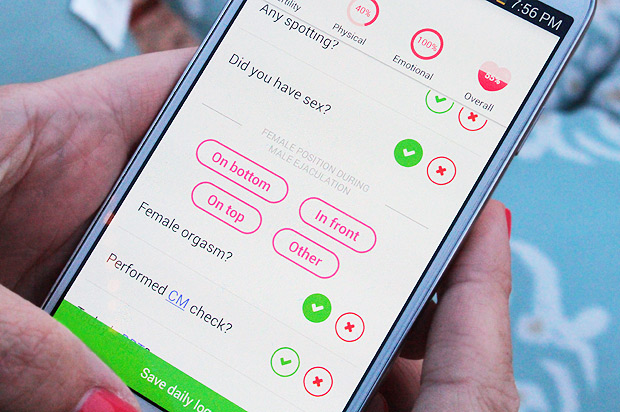
\includegraphics[width=\linewidth]{img/Glow-App-review-screenshot-1.jpg}
	\caption{The Glow application collects a variety of intimate data (image from \cite{glowApp})}
	\label{fig:glow_app}
\end{figure}
Launched by PayPal founder Max Levchin in 2013, the application offers great concurrence with many other fertility and natural prevention apps. Glow can track a huge amount of intimate data, e.g. the menstruation, position and firmness of a woman's cervix, sexual intercourse with the women's position during ejaculation, "whether or not they had an orgasm and whether they experienced emotional or physical discomfort during sex" \cite{doi:10.1080/13691058.2014.920528}. In addition, the mood of the user can be tracked.
The difference to other applications is that Glow makes the collection of intimate data a family affair. The users' partners are invited to download a mirror application and provide additional data \cite{levy2014intimate} The application also sends messages to the partner about the current status of the partner's period, reminding of attentions such as flowers or a nice message.
The data of the female users are evaluated collectively in order to be able to specify better forecasts for the individual user from the large collection.

Danaher et al. \cite{doi:10.1080/15265161.2017.1409823} argue under the point \textit{Gender Relationship Objection}, that these types of technologies are making women an object of surveillance and quantification.
They give the impression that the cycle of a woman is unsupervised chaotic and can only be "rebuilt" with strict control.
In addition, the Glow application would promote the development and enhancement of gender stereotypes, as also augmented in \cite{doi:10.1080/13691058.2014.920528}.
 
The disclosure of such intimate data is questionable if the user disregards how the data is further evaluated. These technologies can be helpful in the evaluation of the collected data, and remind of the daily measurement. Unfortunately, these very sensitive data are also used for commercial purposes.

\subsection{Condition D: Surveillance, Abuse and Revenge}
\label{subsec:D}
The condition D is about surveillance in relationships. The other three conditions are also about surveillance, but in a different way. The differences are briefly described and illustrate in the following.
 
The conditions described above deal with the different situations in which intimate data can be created and used, e.g. for surveillance purposes.
The section \ref{subsec:A} covered the collecting of data via social networks and online dating services. In section \ref{subsec:B} the generation and collection of intimate data in a relationship was described. In section \ref{subsec:c} it was discussed about the monitoring of woman or rather their menstrual cycle and fertility.
A summary of the previous conditions can be seen in figure \ref{fig:intimate_surveillance}.
As described above, users voluntarily or unconsciously disclose this data to benefit from data science (see Glow application, which calculates the course of the menstrual cycle among other analytics from the data set of other users, making a relatively reliable prediction of ovulation possible without the user providing daily tracked information).
In all these states one can speak of an \textit{voluntarily participatory surveillance}.
The supervisor is usually the provider of the smartphone application or the wearable devices, which is commercial interested in the data. This possible form of surveillance is discussed critical in more detail in section \ref{sec:risks}.

In this section the mutual surveillance of the partners in existing or also terminated relationships is considered in more detail. 
The type of surveillance in a relationship can be voluntary or involuntary. The threat of providing such kind of intimate data in the context of an intimate relationship should not be disregarded.
\begin{figure}[htb]
	\centering
	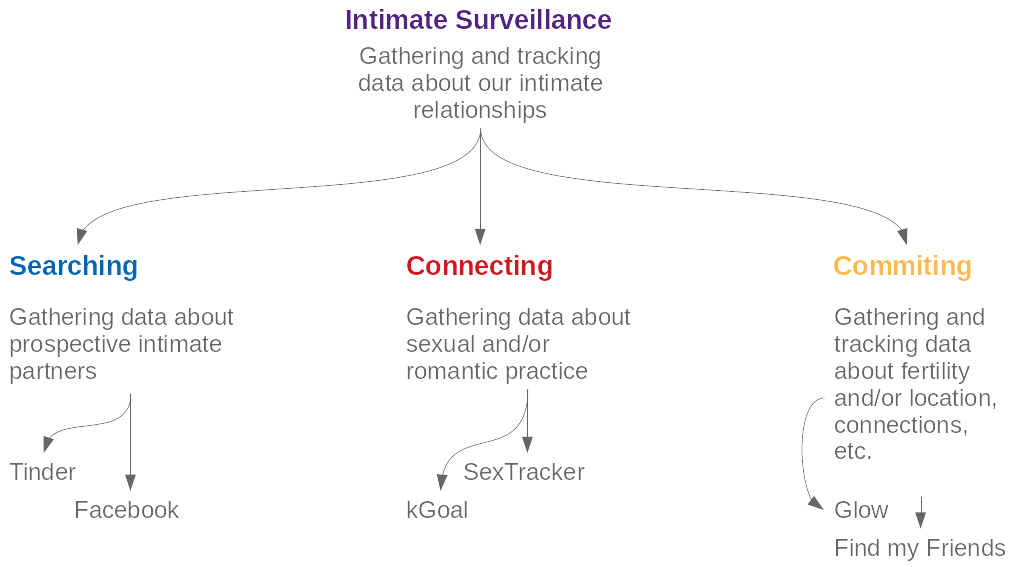
\includegraphics[width=\linewidth]{img/summarizing.png}
	\caption{Surveillance may take place both through applications, social media, etc. and in interpersonal relationships (based on Danaher \cite{ethicsOfSurveillance})}
	\label{fig:intimate_surveillance}
\end{figure}

\subsubsection{Mutual voluntary surveillance provides mutual trust?}
In section \ref{subsec:B} and table \ref{tab:typ_of_QR} the term \textit{intimate surveillance} was already mentioned.
For mutual voluntary surveillance in an existing relationship, Danaher et al. \cite{doi:10.1080/15265161.2017.1409823} have given an interesting but also questionable approach.

The authors consider if mutual voluntary surveillance in an existing intimate relationship could be useful to provide mutual trust.
First they define the concerns related to the use of such \acs{QR}-technology for supporting partner's mutual trust in a well-functioning relationship. They found, that such a tracking technology could corrode the mutual trust, which a romantic relationship is usually based on.

Levy \cite{levy2014intimate} argued that mutual trust in a relationship has played a fundamental role so far and promotes pro-social behavior in the relationship. If digital technologies take on this role now, by tracking the partners in the relationship, and if the partner does control themselves and build their trust on it, it does not rely on loyalty to the partner anymore, but only to the tracking software.

Due to this fact it is questionable where the use of such tracking technologies in relationships leads.
Danaher et al. argued that "even if mutual trust is an ideal, it is an ideal that many fall short of in reality." \cite{doi:10.1080/15265161.2017.1409823}.
The authors suggested that partners, to some part in the relationship, voluntarily observe themselves to appease the other's doubts. But they also added some considerations to privacy and security risks. Such use of tracking technology requires extreme caution and respect. It requires the explicit agreement of the partner. Furthermore, the technology itself should involve a "hard-but-reversible lock-in", to bring the surveillance under control and interrupt this if one of the partners no longer wants to be tracked by the other.
They suggested that an example could be an smartphone application that allow mutual surveillance, e.g. for a period of time.
It would be interesting to survey if partners would use such an tracking technology, in which circumstances and conditions and, especially, if they would find such an approach desirable and helpful in a relationship. 

Some couples are using tracking technology already in their relationship. %TODO: Quelle
There are a few possibilities to do this via the smart phone. The Google Play Store and also the App Store by Apple offers some applications to locate a person, e.g. friends, a family member or the own children. To give an example, with the application called \textit{Find my Friend} it is possible to locate another person which is also using the same application or (if the other person doesn't use a smartphone) with the agreement via a simple text message \footnote{Find my Friends application: \url{https://play.google.com/store/apps/details?id=com.fsp.android.friendlocator}}. After agreement, the users can communicate and locate each other.
One further option to track people who matter most is given via the operating system of the smartphone itself. Apple offers the service called Family Sharing \footnote{Apples Family Sharing: \url{https://support.apple.com/en-us/HT201087}}. With this service the user can share the actual location with members in the family group after the function called \textit{location sharing} is turned on. With the \textit{Find my Friend} application the user can see the location of each members in the family group, if they share their location too.

Another possibility to share a user's location with friends is the \textit{Live Location feature} of WhatsApp\footnote{Live Location feature of WhatsApp: \url{https://faq.whatsapp.com/de/android/26000049/?lang=en}}. With this function a user can share the location with friends for a period of time.

These three examples should only give an overview what is in use today. 
%It is on no case completely. 
It only shows that technologies for location tracking are already available and in use.

\subsubsection{With whom do people track their location?}
Consolvo et al. \cite{Consolvo:2005:LDS:1054972.1054985}  investigated the willing disclosure of information from location-enhanced technology users to specific other people. In this study, 16 participants had given a social network consisting of people from their social networks. This network also includes the participants' partner, in that work called \textit{spouse/significant other}. They found that for the willing disclosure for the user it is most important "[..] who was requesting, why the requester wanted the participants location, and what level of detail would be most useful to the requester.". The results also shows that "[...] who the requester was had the strongest influence on participants willings to disclosure.". If the partner, called \textit{spouses/significant others} was requesting, the participants "[...] were willing to disclosure something for 93\% of the 670 requests.".
It can be concluded, that people use these technologies and are willing to disclosure information about their location, activities and accompaniment. Further they give more details of information if the have an special relation to the requester, such as an intimate one.

\subsubsection{Why do people track their location with others?}
%TODO. Win more trust?

%TODO: Transparency in relationship?
In the opinion of Ikrath \cite{Ikrath2018} we are living in a change of values. The present generation is non-solidarity and self-centered. Individual values are preferred over community values.  
As a result it could be difficult to have a relationship based on trust, similar to Danaher's et al. \cite{doi:10.1080/15265161.2017.1409823} argument.

Also the urge for control could be a possible reason why people are tracking each other.

\subsubsection{Does location tracking corrode the love?}
It is questionable, if location tracking is helpful in a relationship.
Engl et al. \cite{engl2016} actually work on an application with an associated website for partners.
The application should encourage the user to regularly invest time in successful discussions and to improve the communication in the relationship.
In addition, the application gives specified tasks and configurable exercises for reflection and interaction, as well as for assessing the quality of the relationship.
%TODO: Nachfragen, warum?
But the application will be implemented without a location tracking function.

%TODO: Kommunikation

Location traction in a relationship with digital techniques provides some risks regarding to privacy. Below, the possible dangers are considered in more detail.

\subsubsection{Abuse and revenge}
Technologies as discussed above can be misused for other purposes. Freed et al. \cite{freed2018stalker} conducted a study with 89 participants to show how abusers in \ac{IPV} context exploit technologies to intimidate, threaten, monitor, impersonate, or harass their victims.
They grouped the different types of attacks by abusers in four categories. A summary of these categories with examples is shown in figure \ref{fig:abusing_categories}.

\begin{figure}[htb]
	\centering
	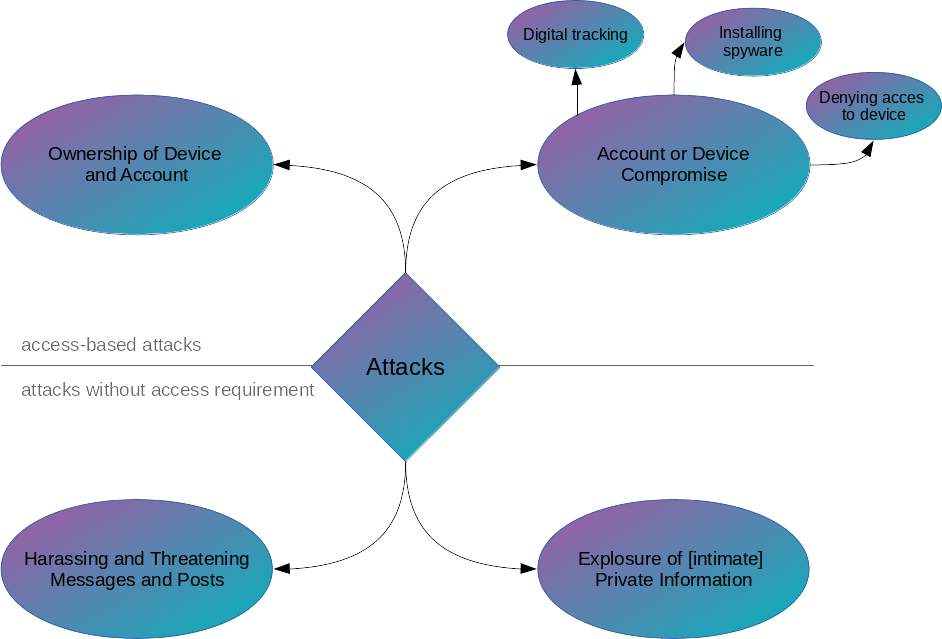
\includegraphics[width=\linewidth]{img/abusing_categories.png}
	\caption{Summary of different types of attacks by abusers in \acl{IPV} context (based on content from Freed et al. \cite{freed2018stalker}).}
	\label{fig:abusing_categories}
\end{figure}
Hereinafter these four categories grouped by Freed et al. \cite{freed2018stalker} are explained in more detail, focusing on intimate data, which the abuser accessed. Freed et al. found also other attacks (e.g. messages, posts in social networks and phone calls) to harm the victim, but that goes beyond the focus in this work.

\textit{Ownership of Device and Account}
Abuser and victim have or had an intimate relationship. This often includes a cohabitation or  marital togetherness. In such a relationship with shared possession one of the partners commonly is taking responsibility for the couple finances. This fact leads to devices and accounts belonging to the abuser.
The study showed that many participants (n=20) stated that their device (e.g. smart phone) was financed by the abuser. 
With the ownership the abuser gained control about the different functions a provider offers to its customers. The abuser was able to control the victims digital accounts, e.g. received the phone bills and therefore knew detail facts about the usage behavior by the victim (including call history, text messages and voice mails), or took advantage of the data back-up services and got information or data, e.g. pictures saved on the victims smartphone. The abuser was also able to use the "[...] location-based services to track victims devices, including anti-theft services (e.g., 'Find My Phone'), parental tracking, and other safety-based services (e.g., Find My Friends') [...]" \cite{freed2018stalker}.

\textit{Account or Device Compromise}
If the abuser was not able to get access through the ownership of devices and accounts, there were also other ways to gain access. The study sowed that "[...] abusers are able to compromise victims' devices or accounts against their will and/or without their knowledge. Such compromises predominantly occurred via two routes: compelled password disclosure and remote compromise of accounts by guessing of victim passwords or the answers to password reset security questions.". If the abuser had access to the device and/or the account, it was no longer difficult to install software for spying the victim.
The study also showed that the abuser were able to gain access to victim accounts by guessing the password or compelling password disclosure. With these access abuser were able to monitor, impersonate and hurt their victims \cite{freed2018stalker}.

\textit{Harassing and Threatening Messages and Posts}
Abuser used social networks to harm their victims. The victims were harassed with messages or calls on the smartphone device. In addition, the networks were used to damage the victims' reputation.
Therefore abuser contacted friends and family of the victims in order to negatively influence the friendship and/or to pursue their jealousy.

\textit{Exposure of Private Information}
Digital technologies offer abusers a way to harm their victims by disclosure private information to third parties or friends and social contacts. Freed et al. found that "[t]he most common exposure-based threat [...] was exposure of intimate images (photos or videos) of victims, commonly known as non-consensual pornography or \textit{"revenge porn"}[...].

Levy also wrote about the \textit{revenge porn} as an possible risk in condition D in the life course of intimate relationships.

Tong surveyed in \cite{Tong2013Facebook} "[...] how [...] individuals use Facebook as a from of surveillance." The survey showed that there were three dimensions for general social activity monitoring. The first was "[...] referred to looking at the ex's profile, photos, and status updates to see what the ex is doing." Second it was important to "[...] detecting an ex-partner's new romantic interests [...]", e.g. by checking the realtionship status of the ex-partner. The third dimension included "[...] direct statements made to, or by the ex-partner [...]".
Compared to the results in the study from Freed et al. \cite{freed2018stalker} mentioned above, these three dimensions seems harmless. However, these activities are also kinds of surveillance that the user, which is monitored, can not control. It is similar to the research results in condition A in \ref*{subsec:A}.

In summary, in \acs{IPV} context abuser are increasingly using digital technology to harm their partner. Freed et al. \cite{freed2018stalker} found that the attacks were technologically unsophisticated and often carried out by a \textit{UI-bound adversary}.











\section{Risks}
\label{sec:risks}
Lupton wrote in \cite{doi:10.1080/13691058.2014.920528} "[...] that mobile digital technologies that can be used for surveillance are part of everyday social life."
Since the technologies discussed in section \ref{sec:consideration_life_course_conditions} are in daily use, they pose some risks to the users privacy, the perception of themselves and also of their relationships.
In this section some of these risks are summarized to give an overview.
The overview is divided into three categories which are described in the following.

\subsection{Quantification: Perception and rating of the self and the relationship}
Due to the various ways in which intimate data can be tracked, there is a risk of losing the actual reference to the data as Luption wrote in  \cite{doi:10.1080/13691058.2014.920528} and \cite{lupton2016quantified}.

In Condition B in \ref{subsec:B} it was mentioned that by tracking of sexual activities the act itself is only perceived by numbers at a later time, thus the act is quantified. The quality and perception of scenes felt by the user can be lost. Or in other words, the user can be lost in a jumble of numbers \cite{kelly2017inevitable}.
When using these technologies, the user should be aware of why he or she is using them and what these data are actually collected for \cite{doi:10.1080/15265161.2017.1409823}. 
Often it is the case that many users are interested in tracking at the beginning, but after a while they gave up using the tracking device and are no long interested in \cite{sjoklint2015complexities}.

In Condition C in \ref{subsec:c} the tracking of the cycle and fertility of female users is described. 
Especially for the sympto-thermal method by Roetzer a digital device to support the measurement and evaluation of the measured values could be helpful. However, it is claimed that the 
analog measurement leads to better results. %TODO: Quelle
Regardless of this, there is also the possibility of losing in the tracked data and not paying attention to one's own body feeling.

This also applies to applications in which advice and tips for the relationship are given in the form of notifications, e.g. by the Glow application mentioned in \ref{subsubsec:glow_application}. It is questionable whether this type of support for the relationship is sustainable or whether it is influencing the self-questioning of the actual relationship status.

\subsection{Trust: Unknowingly and Knowingly Tracking by Intimate Partner}
The risk of being lost in data also applies to data obtained through mutual (location) tracking in relationships described in Condition D in \ref{subsec:D}. This kind of tracking also includes the risk that the focus is solely on the data and the trust on which relationships normally build up is lost. The fact that one knows the exactly location of the partner at every time can lead to wanting constant knowledge about the partners location. What is if the location data is not available once a time? This should be examined in future work.

%The surveillance of the partner without his consent is on the topic of \acs{QR}-Technologien out of the discussion, as Danaher et al. in \cite{doi:10.1080/15265161.2017.1409823} argue. This is clearly the abuse of the data. This includes also the use of such apps as Flexispy \footnote{\url{https://www.flexispy.com/en/}}.

The approach that partners voluntarily monitor each other as described in D could also create problems related to the use of such an application or tracking device.
This includes for instance the abuse by a dominant partner that might force the use of such software in the relationship.
\begin{quote}
Many survivors were unaware that their location could be tracked using these services and asked us to teach them how to turn off location services on their phone. Professionals also described how survivors' lack of awareness regarding location tracking may result in potentially dangerous physical stalking [...]. \cite{freed2018stalker}.
\end{quote}


\subsection{Privacy: Risks related to \acs{QR} technologies}
In Danaher et al. \cite{doi:10.1080/15265161.2017.1422294} the risks associated with the use of \acs{QR}-technologies are summarized.
The authors argued that the concerns " [...] of the privacy-invading elephant lurking in the room [...]" are not alone a problem of a single person, but also involves one or more persons, e.g. a person with which one is sharing knowledge about intimate facts like such in a relationship. In this case it is a exclusively private and an interpersonal matter. The decision whether and with what device \acs{QR} technologies are used in a relationship depends on the person itself.
As further concerns, they stated that users use applications on devices that are also used for other purposes, e.g. such devices as smart phones, and that these devices are connected to the Internet. 
They concluded their argument that it is not a single process of tracking the data, which leads to problems. Rather, the problem lies in the fact that third parties collect the data on the devices that track the data, and so they get the data with existing network connection.

A solution for this concern could be applications on devices which does not communicate with third parties servers via a network connection. This could be devices that only track the data the user want to quantify, without network connection, which lead to use an device in addition to the smartphone.
Or, go a step backwards, the user can track that data completely without digital technologies, e.g. as mentioned above with the sympto-thermal method model by Roetzer.
But the tracking without digital devices is difficult to realize if there is a possibility to support technology tracking. Digital helpers make sense, they are usually reliable and make everyday life easier. Thus, manual tracking is not an alternative.

Users of \acs{QR} technologies, tracking devices, smartphone, social network and others should always be aware of the amount of data which are disclosed and also to whom. Providers and third parties are commercial interested in these data. In addition, the privacy and consent declarations should be noticed and/or simplified, as Anaya et al. in \cite{anaya2018ethical} suggested.

User should also aware whether their data are used for big data science, e.g. with the tracked data in the Glow application.

%TODO: Es fehlt ein UNDO für Datenteilung

Even the usual methods for security arrangements are not sufficient in certain situations. So they are suitable for attacks by strangers, but not for people who are very close and so know many intimate details.
\begin{quote}
	We found that the typical vectors of remote account compromises are technical mundane. Frequently, abusers are able to use their knowledge of the victim's personal details to infer passwords or correctly answer their security questions and reset their password [...]. \cite{freed2018stalker}
\end{quote}


%\section{Discussion}

\section{Conclusion and future work}
\label{sec:conculsion}
%TODO: Summarizing the paper
In this work, different conditions in a relationship  were considered in which intimate data can be searched, collected tracked and shared.
Further, an attempt was made to formulate a definition for the term \textit{intimate data}. It also summarized how people perceive this data and how the data affects their perception.

%TODO: Provide all findings in a short sentence
%\subsection{RQ1: What data is perceived as intimate? In what circumstances?}
Intimate data arises predominantly from intimate activities, e.g. sexual activity and what is related with it, such as sexual preferences, health, etc. Information about sexual preferences is also perceived as intimate. Fertility data, which is more prevalent in healthcare, is perceived as intimate, too. The view of what data is intimate may change, depending on the circumstances. Information shared with the partner until recently can quickly become intimate when the interpersonal relationship breaks down. A precise definition is therefore not so easy to find. What is intimate is partially perceived subjectively. Thus, the personal boundaries of collecting, tracking and sharing data are subjective to the individual too.

%\subsection{RQ2: Why do people track intimate data in relationships?}
Technologies and devices are being used today to simplify processes. In the context of the technologies described above, one can conclude that these are used to obtain more information. In this way one can get to know oneself better, learn more about the body and the  own life. There is also the possibility to communicate these insights with like-minded people.
%\subsection{RQ3: What do they do with, e.g. tracking, storing, sharing and discussing and with whom?}
The collected data are evaluated in the own interest. In some cases, the data are also shared to benefit from the community, whose data are also available (big data science). The data is also shared to compare with others.
There is a possibility that only the data in the form of numbers are noticed, and the intrinsic perception is lost.

%TODO: Own opinion, answering question from intro
A problem may be the change in values in everyday life.
In a romantic relationship a lot of information is shared over time, even those that are very intimate. This is important for the well-being of the relationship, because  trust is based on such shared facts. But at the same time providing such important intimate information can be a point of attack. Nevertheless, this does not means that it is better to hide such intimate information in a romantic relationship and build up relationships based on superficial communication.
Nevertheless it is showed in several works, that abusing such intimate data and information is commonly used and possible. Due to this fact, more awareness for the own intimate data is needed, as well as the knowledge how to protect these data from abusing and disclosure, and how to protect oneself from being monitored involuntary by the partner or third parties.

%TODO: Future work
Condition \ref{subsec:D} includes considerations towards mutual voluntary surveillance in a romantic relationship. One fact by tracking the location of the partner constantly should be noticed in future works: It is questionable if the quantification of trust in romantic relationships is influencing the perception of the partners in the relationship, and in which way. Further is has to be  investigated whether location-based tracking devices are helpful for building trust in a relationship.

\section*{Acknowledgment}
I thank Hanna Schneider and Mariam Hassib for their friendly help and support when writing this paper.

\printbibliography
\end{document}
